Im Gegensatz zur SiSprocom hat die allink einen relativ grossen Kundenstamm.
Das bedeutet, dass kein grosses Klumpenrisiko existiert. Jedoch ist auch
die Auftragskontinuität der einzelnen Kunden viel kleiner. Für manche arbeitet
allink jeden Monat an einem neuen Projekt, für anderen einmal im Jahr.
In der Grafik \ref{pic:kundenauszug} ist ein Teil der Kunden abgebildet.

\begin{figure}[htbp]
\begin{center}

\includegraphics[width=0.73\textwidth,angle=0]{./bilder/analyse/kundenauszug.jpg}
\caption[Kundenauszug von allink]{Kundenauszug von allink\footnotemark}
\label{pic:kundenauszug}
\end{center}
\end{figure}
\footnotetext{Eigene Darstellung}

Unterteilt man die Kunden von allink in die gängigen Firmengrössen Kleinstunternehmen,
kleine Unternehmen und mittlere Unternehmen, so gelangt man zu einer interessanten 
Verteilung. Die Definition der Unternehmensgrössen basiert auf einer Empfehlung
der Kommission der Europäischen Union\footnote{\citealp*[Vgl.][Anhang Art. 2]{eu_komission_unternehmen}}.
Diese unterteilt die Unternehmen nach dem in der Tabelle \ref{tab:eu_unterteilung} 
abgebildetem Schlüssel.

\begin{table}[h]
\begin{center}
    \begin{tabular}{clccccc}
        \toprule \textbf{Typ} & \textbf{Beschäftigte} & & \textbf{Umsatzerlös} & & \textbf{Bilanzsumme} \\
        \midrule Kleinstunternehmen & $<$ 10 & und & $\leq$ 2 Mio \euro & oder & $\leq$ 2 Mio \euro \\
        \midrule Kleine Unternehmen & $<$ 50 & und & $\leq$ 10 Mio \euro & oder & $\leq$ 10 Mio \euro \\
        \midrule Mittlere Unternehmen & $<$ 250 & und & $\leq$ 50 Mio \euro & oder & $\leq$ 43 Mio \euro \\
        \bottomrule
    \end{tabular}
    \caption[Empfehlung Unternehmensunterteilung, Kommission der Europäischen Union]{Empfehlung 
        Unternehmensunterteilung, Kommission der Europäischen Union\footnotemark}
    \label{tab:eu_unterteilung}
\end{center}
\end{table}
\footnotetext{Eigene Darstellung mit Anlehnung an \citealp*[Anhang Art. 2]{eu_komission_unternehmen}}

Die Kategorisierung der Kunden, abgebildet in der nachstehenden Grafik \ref{pic:kundenkategorisierung},
basiert überwiegend auf den Informationen von moneyhouse\footnote{moneyhouse bietet Handelsregister- und Firmendaten, \url{http://www.moneyhouse.ch}}, 
da man nicht alle Kunden um aktuelle Mitarbeiter- und Umsatzzahlen bitten konnte.
Zusätzlich zu den in der Tabelle \ref{tab:eu_unterteilung} aufgelisteten Kategorien 
wurde noch die Kategorie ``Grosse Unternehmen'' hinzugefügt, um Firmen mit genau 
oder mehr als 250 Mitarbeiter kategorisieren zu können.

\begin{figure}[htbp]
\begin{center}
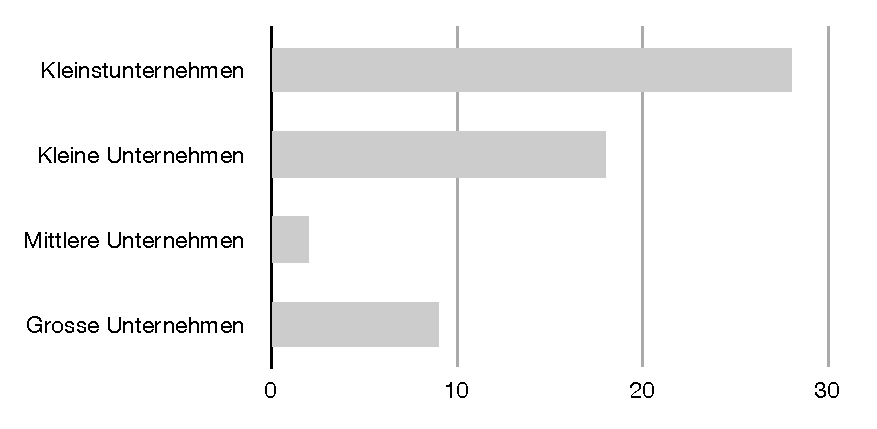
\includegraphics[width=0.75\textwidth,angle=0]{./bilder/analyse/kundenkategorisierung.pdf}
\caption[Anzahl Kunden der allink in Unternehmensgrössen kategorisiert]{Anzahl 
    Kunden der allink in Unternehmensgrössen kategorisiert\footnotemark}
\label{pic:kundenkategorisierung}
\end{center}
\end{figure}
\footnotetext{Eigene Darstellung}

Es wird absichtlich nicht die vollständige Liste der Kunden von allink und deren 
Kategorisierung beigelegt, da allink nicht alle Kunden in dieser Arbeit namentlich 
aufgelistet haben möchte. Bei Bedarf kann die Liste aber bei allink eingesehen werden.

Wie man erkennen kann, arbeitet allink überwiegend mit Kleinst- und kleinen 
Unternehmungen zusammen. Interessanterweise auch mit mehr grossen als mittleren
Unternehmen. Die verschiedenen Firmenkulturen der Kunden haben auch einen 
Einfluss auf die Projektabläufe. Grundsätzlich stellen sich wohl alle Kunden
der Herausforderung, ihre Projekte gut zu organisieren. Je nach Auflagen oder
Abläufe der Kunden, hat dies auch Auswirkungen auf den Projektablauf der allink.
Deshalb wäre es falsch anzunehmen, dass sie zur Zeit bei jedem Projekt und 
Kunden das selbe Vorgehen anwenden können.

Möglicherweise genau deshalb existiert zur Zeit kein definierter Projektablauf. 
Doch gibt es klar erkennbare Gemeinsamkeiten über alle Projekte, bzw. Projektabläufe.
Im nächsten Kapitel \ref{chap:projektablauf} wird versucht, den heutigen Projektablauf so 
abzubilden, dass er für die meisten vergangenen Projekte Gültigkeit hat.
